\section{Chapter 1}

\subsection{Donald Hebb} 
Organization of behaviour - 1949 learning mechanism:
\begin{itemize}
	\item When an axon of cell A is near enough to excite a cell B and repeatedly or persistently takes part in firing it, some growth process or metabolic change takes place in one or both cells such that A's efficiency, as on of the cells firing B, is increased.
	\item As A repeatedly excites B, its ability to excite B improves.
	\item Neuron that fire together wire together.
\end{itemize}

\subsection{Hebbian Learning}
\begin{itemize}
	\item If neuron $x$ repeatedly triggers neuron y, the synaptic knob connecting $x$ to $y$ get larger.
	\item In mathematical model:
	\[ w_{xy} = w_{xy} + \eta xy \]
	\item Weight of the connection from input neuron $x$ to output neuron $y$.
	\item This simple formula is actually the basis of many learning algorithms in machine learning.
\end{itemize}

This idea however is fundamentally unstable:
\begin{itemize}
	\item Stringer connections will enforce themselves.
	\item No notion of "competition".
	\item No \textit{reduction} in weights.
	\item Learning is unbounded.p
\end{itemize}

People came up with all kinds of modifications for it to try to make it more stable:
\begin{itemize}
	\item Allowing for weight normalization.
	\item Forgetting
\end{itemize}
This lead to the Generalized Hebbian learning, aka Sanger's rule where the contribution of input is \textit{incrementally distributed} over multiple outputs.
\[ w_{ij} = w_{ij} + \eta y_j\left( x_i -	\sum_{k=1}^{j}	w_{ik}y_k																									\right) \]

\subsection{A better model}
Frank Rosenblatt
\begin{itemize}
	\item Psychologist, Logician
	\item Inventor of the solution to everything, aka Perceptron
\end{itemize}

\paragraph{Original perceptron model}
Consider the eye structure:
\begin{itemize}
	\item Groups of sensors on retina combine into cells in association in the \textbf{projection area}.
	\item Groups of \textbf{projection area} combine into Association cells in \textbf{association area}.
	\item Signals from \textbf{association area} cells combine into response cell \textbf{R}.
	\item All connectioons may be excitatory or inhibitory.
\end{itemize}

Rosenblatt's perception model can then be further simplified:
\paragraph{Simplified perceptron model}

\begin{figure}[h]
	\centering
	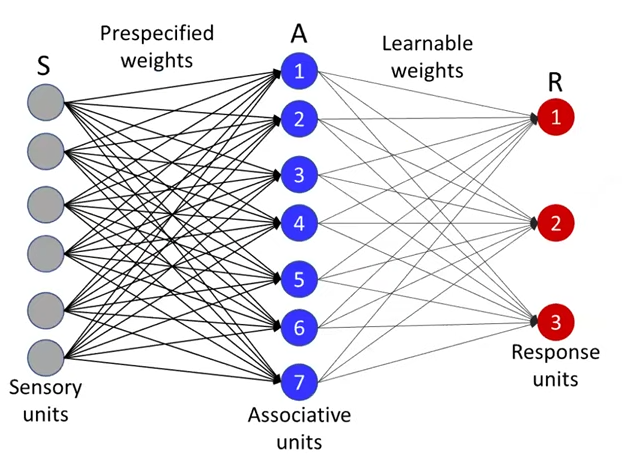
\includegraphics[scale=0.5]{simplified_perceptron_model}
\end{figure}


\begin{itemize}
	\item Association units commbine sensory input with fixed weights.
	\item Response units combine associative units with learnable weights.
\end{itemize}